\documentclass[linenumbers, twocolumn]{aastex631}


\newcommand{\vdag}{(v)^\dagger}
\newcommand\aastex{AAS\TeX}
\newcommand\latex{La\TeX}

\begin{document}

\title{Characterizing the Milky Way and M31 Halo Remnant Shape}



\author[0000-0002-2527-8899]{Mika Lambert}
\affiliation{Steward Observatory and Department of Astronomy, University of Arizona, 933 N. Cherry Ave., Tucson, AZ 85721, USA}

\received{\today}

\begin{abstract}

N-body simulations of the Milky Way and Andromeda galaxies can be used to predict the fate of not only the baryonic matter but also their dark matter halos. 
Our current understanding of dark matter is still uncertain, therefore modeling the evolution of the dark matter halos of these galaxies will help us constrain the properties of such mysterious particles. 
Specifically, defining the shape of the halo remnant is of one the main characteristics we want to explore. 
Determining the shape of the halo remnant means we can extrapolate our result to other galaxies with known halo mass distributions and compare if our models are consistent.
We found that the shape of the halo remnant is triaxial with the axis in the x-y plane being the longest with an axis ratio of 1.129, followed by the x-z plane with an axis ratio of 0.91, then the y-z plane with an axis ratio of 0.885. 
Our finding indicates that the density profile of the dark matter halo remnant is affected by the major merger event which changed its shape.

\end{abstract}

\keywords{Dark Matter Halo, Halo Shape, Cold Dark Matter Theory, Galaxy Merger, Merger Remnant }

%% Keywords should appear after the \end{abstract} command. 
%% The AAS Journals now uses Unified Astronomy Thesaurus concepts:
%% https://astrothesaurus.org
%% You will be asked to selected these concepts during the submission process
%% but this old "keyword" functionality is maintained in case authors want
%% to include these concepts in their preprints.
%\keywords{Milky Way,  M31, Dark Matter Halo} 

\section{Introduction} \label{sec:intro}

% introduce topic
The two most massive bodies in the Local Group (LG) are the Milky Way (MW) and the Andromeda Galaxy (M31). The fate of these objects is an important part of understanding galaxy evolution and mergers because we can study their kinematics and mass profiles in great detail as they evolve. 
% CDM theory
The interaction between these objects will also help us explore the cold dark matter paradigm. Since the construction of the $\Lambda$CDM model, we believe these dark matter particles that weakly interact with baryonic matter make up $\sim$ 27\% of the matter in the universe \citep{2014LCDM}. This dark matter forms complex structures in which galaxies reside called dark matter halos. 
% halo shape
The halo shape, as in the three-dimensional distribution of the mass of the halo, is also an important characteristic of the dark matter.
% dark matter halo
The mass profiles and shape of these dark matter halos around galaxies will shed light on their effect on the baryonic material.
%galaxy merger 
Major galaxy mergers require the sizes of the galaxies to be comparable enough to cause the morphology of the baryonic matter to evolve after a collision.
Major mergers, like the predicted merger between the MW and M31, are especially intriguing due to the multitude of dynamic processes occurring and the significant change in morphology of the merger remnant as a result. 
% merger remnant
The end product of the major merger is called the merger remant which occurs when the baryonic matter has dynamically relaxed.
The merger remnant's halo may also have significant differences from the initial galaxies' halos as well.

% why the topic matters
%\subsection{Why this topic matters to our understanding of galaxy evolution}
% what is a galaxy? and galaxy evolution
As M31 is the closest galaxy to the MW, our knowledge of that galaxy is greater than most other extragalactic objects in the universe. Galaxy evolution, which is the process of changing the morphology and composition of galaxies \citep{2004galaxyevolutiondef}, is impossible to observe over human timescales, however, we can predict their evolution using N-body simulations.
N-body simulations of the merger event between the MW and M31 have accelerated our understanding of galactic merger events which have been hypothesized to be the source of the formation of high-mass elliptical galaxies. 
Understanding the profile of the halo remnant will further aid our quest to understand the behavior of cold dark matter because what categorically separates a galaxy from a star cluster is not being able to characterize its properties based solely on its baryonic matter \citep{2012Galaxydef}.
The resulting density profile from our experiment could also be compared to galaxies in more clustered environments that are believed to be the result of mergers. This would shed light on the differences between mergers in the field versus in dense environments.
Further research could also be done on higher redshift galaxies (z $>$ 1) to look at early galaxy formation and merging.
\begin{figure}[ht]
    \centering
    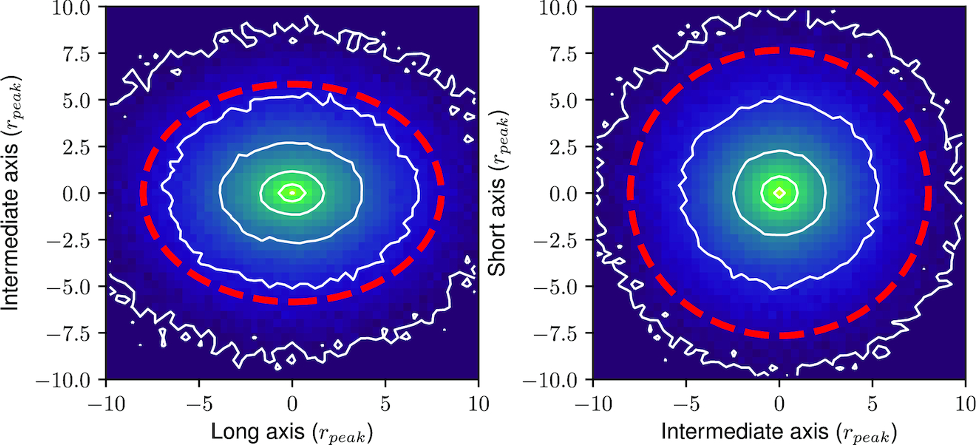
\includegraphics[scale=0.5]{figures/drakos_fig_6.png}
    \caption{The density contours of the simulated remnant halos are in white, and the measured shape ratio is shown in red from \cite{2019drakos}. We see a clear difference in axis ratio between the two different panels.}
    \label{fig:drakos}
\end{figure}

%\subsection{Our current understanding of the topic}
According to \cite{2012VanDerMarel} the next major cosmic event to happen in the Local Group (LG) is the merger of the MW and M31 in $\sim$ 5 Gyrs. 
This event will not only change the physical shape of the baryonic matter of the LG, but also the dark matter halos of the galaxies.
We currently know that for equal-mass mergers, the shape of the halo remnant is dependent on the way the galaxies merge because the merger axis dictates the elongation shape, and the size of the remnant is related to the total energy of the merger \citep{2019drakos}. 
Another interesting aspect of the halos is the concentration of dark matter.
Modeling the density distribution of dark matter halos of galaxies is well defined by the Navarro-Frenk-White (NFW) profile \citep{1996NFW}. Visualizing the density profile of the halos using contour lines shows us the concentration of dark matter as seen in Figure \ref{fig:drakos}.
Astronomers also use simple relations between the mass of a galaxy's halo and its stellar mass using abundance matching \citep{2018Wechsler}. Abundance matching is the assumption that the halo mass is directly correlated to the stellar mass.

%\subsection{Open questions in the field}
There are still many open questions within the realm of galaxy halo remnants.
More complex N-body simulations should be conducted accounting for the satellite galaxy's influence on the merging process. Also, the halos of dense galaxy clusters are still not well defined \citep{2019drakos}. 
We can use these galaxy halos as laboratories for directly and indirectly detecting dark matter particles. An example of direct detection would be using our position in the MW to come across dark particles using facilities like LIGO, and indirect detection would search for the radiation produced by decaying dark matter particles \citep{2012Frenk_White}. In our own LG, the shape of the mass distribution of the merger remnant's halo would be an interesting question to pursue because we can apply our knowledge of this halo remnant to other galaxies and, in the future, build up statistics which could be used to predict the evolution of galaxy halos.


\begin{figure*}
    \centering
    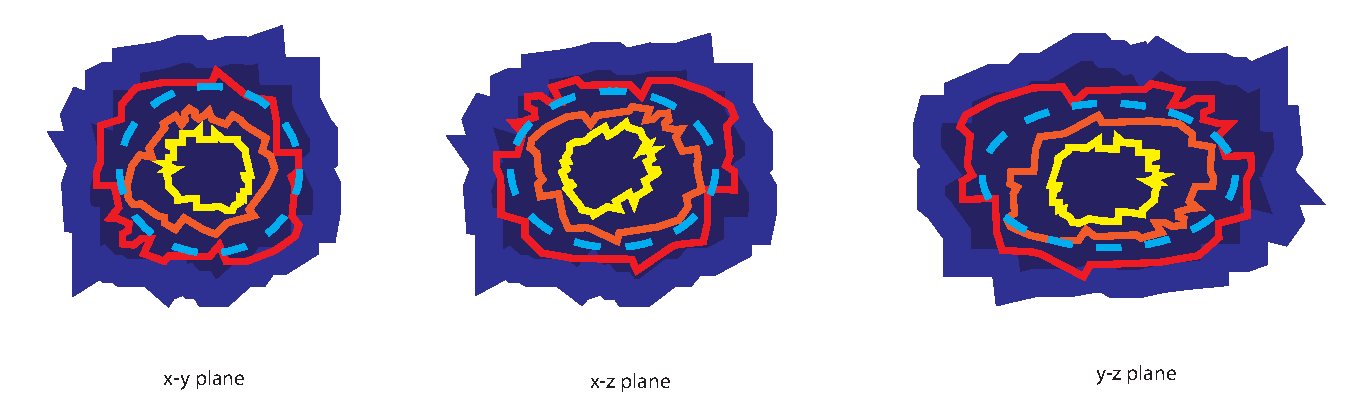
\includegraphics[width=\textwidth,height=5cm]{figures/ASTR400B_project_diagram.pdf}
    \caption{The expected results from our methodology. Left: The halo remnant from the MW-M31 merger with density contours at 1$\sigma$ (yellow), 2$\sigma$ (orange), and 3$\sigma$ (red). The blue dashed line represents the ellipse with a projected axis ratio that appears to fit the halo distribution at the 2$\sigma$ isodensity contour. Middle: The x-z plane of the simulated halo remnant. Right: The y-z plane of the halo remnant with the same identifications as the other panels. We hypothesize that the halo will be triaxial so each axis ratio for each plane is different.}
    \label{fig:method_fig}
\end{figure*}



\section{This Project} \label{sec:project}
In this paper, we will be investigating the change in the 3-dimensional shape of the dark matter halo distribution from the MW halo to the MW and M31 merger remnant halo using the N-body simulation data from \cite{2012VanDerMarel}. 
Looking at the different axes of the distribution, We will determine whether the resulting halo is spheroidal or elongated. 
We will describe the shape of the halo based on whether the shape is prolate, oblate, or triaxial which refers to the direction of flattening of the spheroidal objects.
We will quantitatively investigate the elliptical shape of the 2D projections of the halo in the three planes and characterize their semi-major and semi-minor axes by fitting ellipses to the 2$\sigma$ isodensity contour line.
%2. Is the 3D dark matter distribution spheroidal? or elongated like an ellipsoid? What do terms like prolate, oblate, or triaxial halos mean? https://astronomy.com/news/2010/ 01/astronomers-map-the-shape-of-galactic-dark-matter



%which question from above does this address
This will address the open question in the field that asks what is the mass distribution of the MW and M31 merger remnant's dark matter halo shaped like. The LG is a unique environment to be studying the halos of these objects because they are located in the field and both the MW and M31 are neither red and dead galaxies nor blue and star-forming galaxies. Being able to compare the MW and M31 halo remnant to dark matter halo simulations of galaxies of different colors and environments diversifies our understanding of halo evolution.



%why is this important for galaxy evolution? How will our study help address this open question?
Simulating the merger of these galaxy halos is important to galactic evolution as a whole because major mergers are essential to changes in galaxy morphology due to intense periods of star formation and inevitable quenching, yet it is still not fully understood what happens to the dark matter particles during a merger. Examining the physical shape of the dark matter halo remnant may open avenues to look into probing why the remnant is the shape it is, how dark matter interacts with itself, and if it correlates to the baryonic matter. Similar to how the galactic morphology of the baryonic matter is visually classified, we may start to see a pattern of simulated halos that we can categorize.


\section{Methodology} \label{sec:methodology}

% introduce the N-body simulations
The N-body simulation used in this study is from \cite{2012VanDerMarel}. They considered only stars and dark matter particles that were collisionless and used the hydrodynamic code, GADGET-3 \cite{GADGET2005}. The simulation does not account for gas since it is only a small fraction of the total mass of the galaxy. This also allows for more star and dark matter particles and the simulations are at high resolution for those characteristics. The simulation begins at the current epoch and has 800 snapshots. Each snapshot corresponds to the following relation to calculate the time: Snapshot$*10/.7$ = time (Myrs).


In order to characterize the shape of the halo remnant we use the following approach.
First, we will need to probe the shape of the spatial mass distribution of the MW halo at snapshot 0 using a 2D histogram along all three axes to investigate any non-spheroidal attributes it may have. To do this, we will implement the code from Lab 7 to create the density contours, and we will also need to rotate the position vectors so that the halo's angular momentum is aligned with the z-axis. We will look at the x-y plane, the x-z plane, and the y-z plane distributions for any elongation. Using an ellipse function to fit the contour lines, and we will calculate the semi-major and semi-minor axes. We will also use visual checks to confirm the ellipse is a reasonable  estimate of the contour line.
We will do a similar procedure for the MW-M31 halo remnant using snapshot 700 using a 2D histogram along the three axes and look for prolate or oblate features by looking at the x-y plane, the x-z plane, and the y-z plane. We use snapshot 700 because a snapshot value of 700 gives a time of 10Gyrs. This is where we define the merging galaxies to be relaxed dynamically, and the stars from the MW and M31 are well mixed according to \cite{2012VanDerMarel}. If only one of the planes shows elongation while the other two are equal in size, we will assume the shape is more prolate. If two of the planes show elongation in equal amounts, we will assume the distribution is more oblate. If all three planes are relatively circular, then we will assume the halo remnant distribution is spheroidal. If we see that the axes are different in all three planes we will assume the shape is triaxial. We will also estimate the ellipsoidal measurement of the semi-major and semi-minor axes for the remnant.
The density contours seen in Figure \ref{fig:method_fig} show how concentrated the mass of the halo is. The blue line is the estimated projected ellipse for the corresponding plane. We will use visual checks to determine what the estimated axis ratio is.

\begin{figure*}
    \centering
    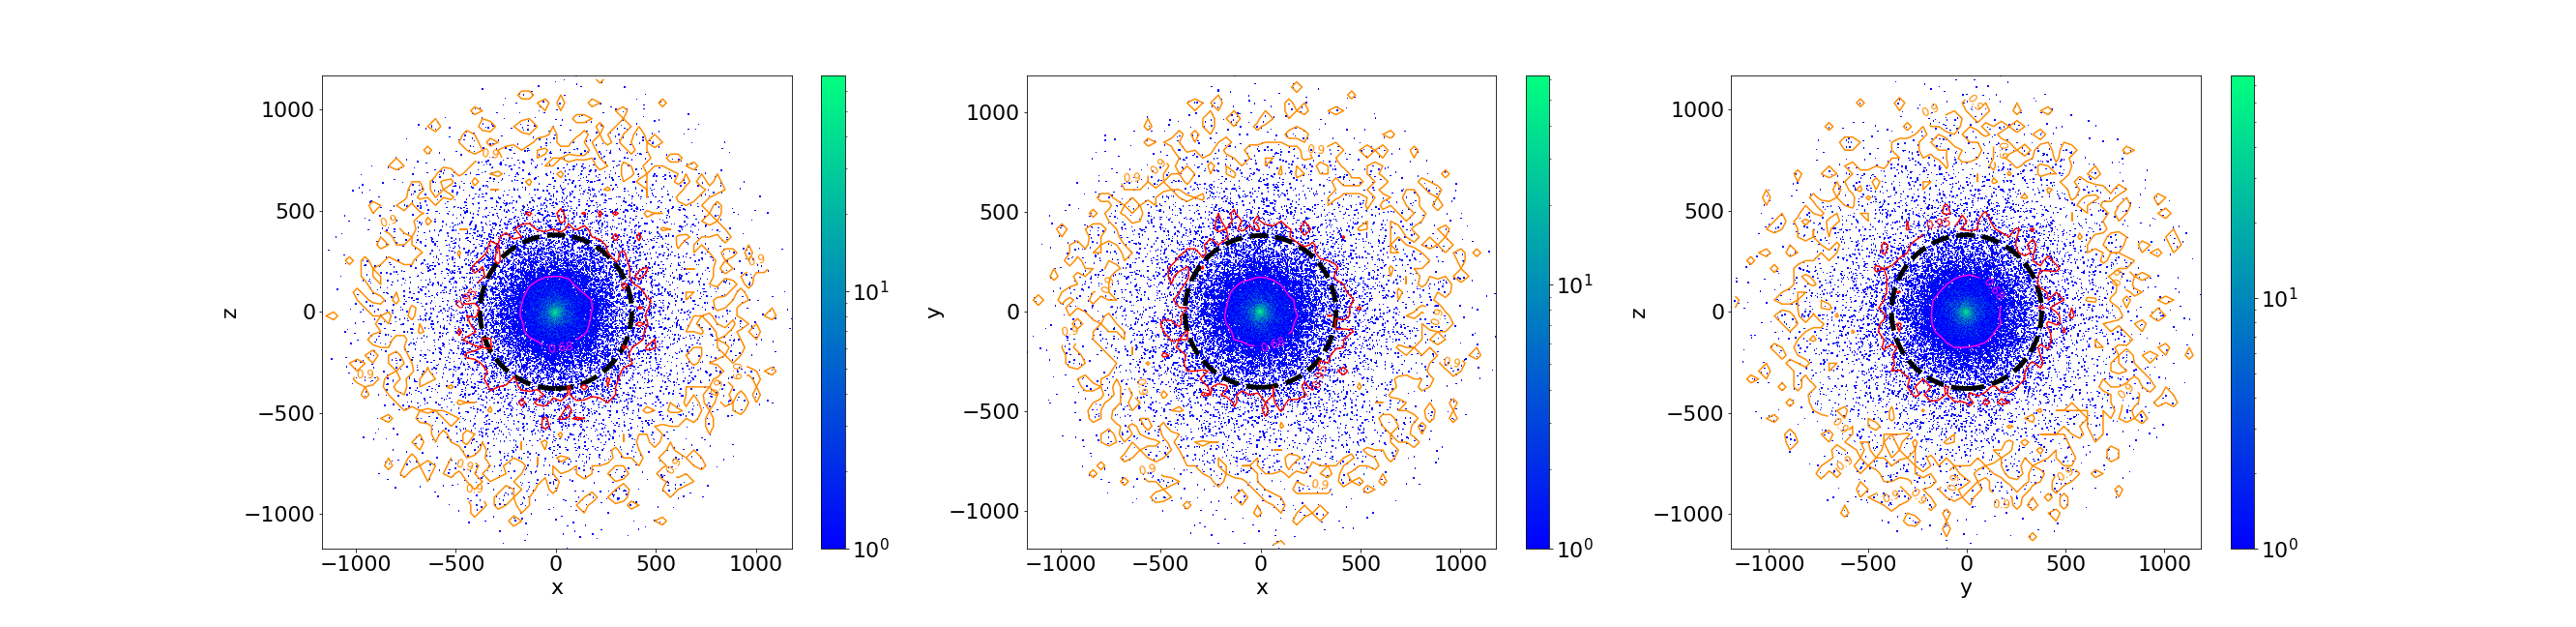
\includegraphics[width=\textwidth,height=4.2cm]{figures/MW_M31_000_3subplots_Density.png}
    \caption{Density contours of the MW at snapshot 0 with the particle density shown in a blue-to-green gradient. The yellow line is the 1-$\sigma$ contour.The red line is the 2-$\sigma$ contour. The pink line is the 3-$\sigma$ contour. The black dashed line shows the modeled ellipse using the 2-$\sigma$ contour as a reference. Left: shows the x-z plane. Middle: shows the x-y plane. Right: shows the y-z plane. We see the ellipsoidal shape in each plane is relatively circular.}
    \label{fig:MW_contour_0}
\end{figure*}

\begin{figure*}
    \centering
    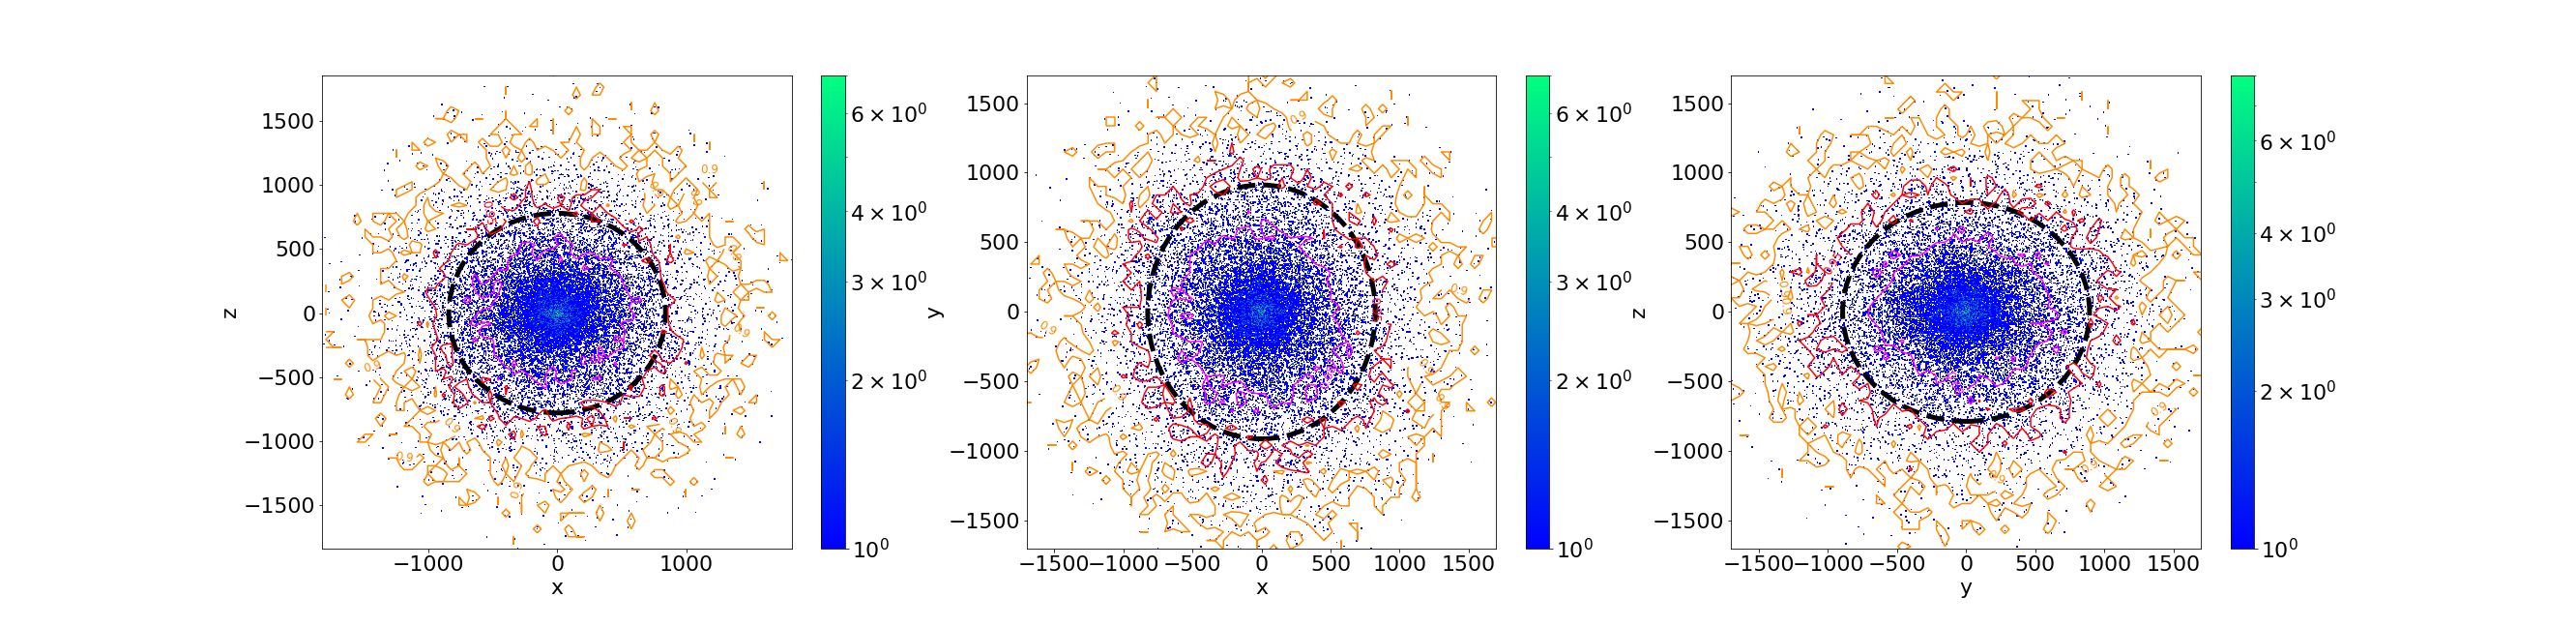
\includegraphics[width=\textwidth,height=4.3cm]{figures/MW_M31_700_3subplots_Density.png}
    \caption{Density contours of the MW and M31 halo particles at snapshot 700 with the particle density shown in a blue-to-green gradient. The yellow line is the 1-$\sigma$ contour.The red line is the 2-$\sigma$ contour. The pink line is the 3-$\sigma$ contour. The black dashed line shows the modeled ellipse using the 2-$\sigma$ contour as a reference. Left: shows the x-z plane. Middle: shows the x-y plane. Right: shows the y-z plane. We see the ellipsoidal shape in each plane has deviated significantly from the ellipse in \ref{fig:MW_contour_0}. We see in both the x-y and y-z planes the ellipsoid has stretched along the y-axis.}
    \label{fig:MW_M31_contour_700}
\end{figure*}

We will create an additional function that creates an ellipse with $\tt{matplotlib}$ using the 2$\sigma$ contour as a reference for comparing snapshot 0 to 700 to be consistent at the same density. This function will also calculate the semi-major and semi-minor axes which will give us quantitative measurements of the shape of the halo. First, we calculate the covariance of the two coordinates, then we normalize them which gives us the Pearson Correlation Coefficient (p). Lastly, we can calculate the horizontal and vertical radius using $sqrt(1+p)$ and $sqrt(1-p)$ respectively and multiply by two times the standard deviation in each direction to get the 2-$\sigma$ density contour level. Then, we multiply by two to obtain the semi-major and semi-minor axes. After that, we can plot the ellipse using $\tt{matplotlib}$ with these given parameters.
To track the evolution of the axis ratio we will need to loop over this ellipse function for each plane at every twentieth snapshot.

We will first be creating plots similar to \ref{fig:method_fig}. We will have two sets of plots, one at snapshot 0 of the MW halo in the x-y, x-z, and y-z planes with the modeled ellipse overlaid, and one at snapshot 700 of the combined MW and M31 halo in the x-y, x-z, and y-z planes with the modeled ellipse overlaid to determine their axis ratio. We will also create a plot of the evolution of the axis ratio for the MW particles in each of the three planes over time from snapshot 0 to 700. We will use every twentieth snapshot, which corresponds to 0.286 Gyrs to get a general sense of how the halo shape evolves with time. This halo shape will focus on the MW particles because adding the M31 particles will not dramatically change the axis ratio of the evolving remnant. Theoretically, if one were to include M31's particles to this axis ratio evolution plot, they would need to consider the point in time where they can say M31 and the MW particles are well mixed which would not occur until snapshot 700 based on our assumptions. 


%\subsection{Hypothesis} \label{sec:hypothesis}
As seen in Figure \ref{fig:drakos} for the merger between two equal-mass galaxies, we would expect a similar shape to emerge from the halo of the MW-M31 halo remnant which is more triaxial than spheroidal with one long axis and two short axes similar to Figure \ref{fig:method_fig}, although Figure \ref{fig:method_fig} shows a more oblate shape.
Prolateness also depends on the amount of mass loss, so in the future, one can use our result to estimate the amount of mass that would no longer be under the gravitational effects of the remnant.
We also expect the axis ratio to become less symmetric over time as the merger happens.

\section{Results}

\begin{figure}[ht]
    \centering
    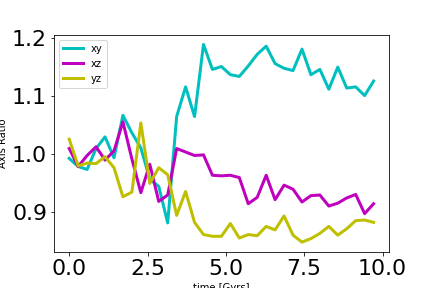
\includegraphics[scale=0.5]{figures/AR_plot.png}
    \caption{The axis ratio versus time in Gyrs for the MW halo particles. The cyan line shows the axis ratio in the x-y plane, the magenta line shows the axis ratio in the x-z plane, and the yellow line shows the axis ratio in the y-z plane. This figure shows all the planes starting with an axis ratio close to 1 at a time corresponding to present day, and significantly deviating by 10 Gyr.}
    \label{fig:AR_evol}
\end{figure}

% MW 000 figure 3 sentences
We note that we are analyzing the inner region of the halo because that is where the bulk of the mass is. The particles seen in Figure \ref{fig:MW_contour_0} and \ref{fig:MW_M31_contour_700} are within one standard deviation of the center of mass of the halo.
Figure \ref{fig:MW_contour_0} shows the initial shape of the MW halo at the present day is relatively circular. This is what we expect because the MW hasn't gone through any major mergers that would disrupt the shape of the halo. 

% snap 700 fig 
Figure \ref{fig:MW_M31_contour_700} shows the shape of the MW and M31 halo remnant 10Gyrs in the future. There is a visual difference in the ellipses drawn at the 2-$\sigma$ contour for all three planes. The x-z and y-z planes show the horizontal axis of the ellipse has increased while the ellipse modeled in the x-y plane has a larger vertical axis compared to Figure \ref{fig:MW_M31_contour_700}. This shows the major merger between the MW and M31 clearly affected the shape of the halo to be a more prolate ellipsoid.


% AR evolution
In Figure \ref{fig:AR_evol}, we see how the axis ratios of the 3 different planes of the MW halo density evolve from the present day to 10 Gyrs in the future. The axis ratio is defined to be the semi-minor axis divided by the semi-major axis (b/a). We see the x-y plane evolved from a relatively circular ellipse with an axis ratio of 1 to and axis ratio of 1.129. This means the semi-minor axis is 1.129 times larger than the semi-major axis which is consistent with what we see visually in Figure \ref{fig:MW_M31_contour_700}. The axis ratio of the ellipse modeling the density of the x-z plane starts at 0.983 and ends at 0.91 which means the semi-minor axis is 0.91 times the semi-major axis which, again, is consistent with the left panel of Figure \ref{fig:MW_M31_contour_700}. Finally, the axis ratio of the modeled ellipse of the density of the y-z plane starts at 0.980 and in 10 Gyrs will be 0.885, also consistent with \ref{fig:MW_M31_contour_700}. This indicates that the halo will evolve into a triaxial shape after the major merger.

\section{Discussion}
% summarize result, does it agree with hypothesis, how does it relate to existing work, importance for galaxy evolution
Using the N-body simulations, our results show that the shape of the MW-M31 halo remnant 10 Gyrs from now will be triaxial because each axis will be a different length. The longest axis will be in the x-y plane, then the x-z plane and y-z plane will follow in size. Although the shape is triaxial in nature, the shape will have a prolateness to it since the x-y plane's axis is significantly longer than the other two.
Our analysis supports our hypothesis that the shape of the halo evolves to be triaxial. In Figure \ref{fig:AR_evol} we see that by $\sim$9 Gyrs, the axis ratios for the x-y plane and y-z plane are tending back towards 1, which makes sense because as time progresses the shape of the halo will eventually relax similar to what the baryonic matter will do. Our claim that the axis ratios will become less symmetric over time as the merger happens is not supported by this result. In the future, it would be interesting to investigate the time at which the halo returns to a completely spherical shape.
This analysis is in agreement with the \cite{2019drakos} simulations for equal-mass objects where their experiment resulted in a triaxial shape as well (see Figure \ref{fig:drakos}).
This is important for galaxy evolution as a whole because understanding how the halo of the merger remnant between the MW and 31 galaxies evolves may aid our understanding of other galaxy mergers. Also, if we can predict the nature of the dark matter particles, we are one step closer to solving the dark matter paradigm. 
Our results also provides context when astronomers assume dark matter halos are perfectly spherical to compute their simulations. Any potential discrepancies between simulated data and theoretical models may be caused by this triaxial shape of the halo; assuming a spherical halo also loses information that comes from the direction of prolateness/oblateness including the direction of a major merger event.

% uncertainties
In Figure \ref{fig:AR_evol} we did not include M31 particles which may have had a slight effect on the axis ratios because the 2$\sigma$ isodensity contour level will be in a different position than for just the MW particles. 
Also, the ellipse function cannot plot ellipses that are at an angle from the horizontal axis, so if there was a tilt in the density contour we could not measure it which means our measurements are a lower limit to the true axis ratios.

\section{Conclusion}
%summarize intro
The use of N-body simulations of the Milky Way and Andromeda galaxies  to predict the fate of not only the baryonic matter but also the dark matter halos has increased in the past several years. 
Due to our current lack of knowledge about dark matter, modeling the evolution of the dark matter halos of these galaxies will help us constrain the theoretical properties of them.
We explored the shape of the halo remnant compared to the initial shape of the MW halo.
Our results can be used in the field to compare to other observed dark matter halos and we will be able to determine if the models are consistent.

% results with hypothesis
We found that the shape of the halo remnant 10 Gyrs from present day will be triaxial in shape. 
The axis in the x-y plane will be the longest, then the x-z plane, and the y-z plane will have the shortest axis. 
The axis ratio of the x-y plane is the significantly larger than the other two (1.129 versus 0.91 and 0.885) which points to a slight prolateness.
Our results agree with our hypothesis that the halo would be triaxial. 


% future
In the future we would like to see if the axis of prolateness is associated with the direction the MW and M31 collide. 
It would also be interesting to explore how well the density profile is fit to a Hernquist profile.
If the simulations extended to farther times, we could investigate the timescales for which the halo remnant will evolve back to a spheroid shape. Including the angle at which the ellipse can be drawn would also improve our results.



\section{acknowledgements}
We acknowledge support from Dr. Gurtina Besla for her guidance and detailed outline for this study, Hayden Foote for troubleshooting code, Aidan DeBrae for his assistance with the ellipse function, and the python packages below.
This research made use of NumPy \citep{harris2020array} This research made use of matplotlib, a Python library for publication quality graphics \citep{Hunter:2007} This research made use of Astropy, a community-developed core Python package for Astronomy \citep{2018AJ....156..123A, 2013A&A...558A..33A}.

\bibliography{sample631}{}
\bibliographystyle{aasjournal}

%% This command is needed to show the entire author+affiliation list when
%% the collaboration and author truncation commands are used.  It has to
%% go at the end of the manuscript.
%\allauthors

%% Include this line if you are using the \added, \replaced, \deleted
%% commands to see a summary list of all changes at the end of the article.
%\listofchanges

\end{document}

% End of file `sample631.tex'.
